
% slides for Ph.D students day

\documentclass{beamer} % oral talk
%\documentclass[trans]{beamer}  % paper version
\mode<presentation> {
  %\usetheme{Darmstadt}
  \usetheme{Madrid}
  \usecolortheme{crane}
  %\usetheme{Goettingen}
  %\usecolortheme{wolverine}
  \setbeamercovered{transparent}
  %\useoutertheme{sidebar}
}
\usepackage{graphicx}
\usepackage{xspace}
\usepackage[dvips]{epsfig}
\usepackage{xmpmulti}
\usepackage{color}
\usepackage{colortbl}
\usepackage{setspace}
\usepackage{array}
\usepackage{latexsym}
\usepackage{comment}
\usepackage{amssymb,amsmath,amsthm}

\usepackage {bussproofs}
\bottomAlignProof

\usepackage{dednatcol}
\usepackage{alltt}
\usepackage[latin1]{inputenc}
\usepackage{times}
\usepackage[T1]{fontenc}
\usepackage[english]{babel}

\definecolor{Blue}{rgb}{0.1,0.1,0.8}

\newcommand{\keywd}[1]{\textbf{#1}}

\setbeamercovered{dynamic}
\setbeamertemplate{theorems}[numbered]

\newcommand{\hs}{\hspace{1cm}}
\newcommand{\vs}{\vspace{1cm}}
\newcommand{\vsfive}{\vspace{5mm}}
\newcommand{\hsfive}{\hspace{5cm}}

\newcommand{\mboxfill}{\mbox{ }\hfill}

% Variables logiques

\newcommand{\rv}{\bleu {rv}\xspace}
\newcommand{\re}{\bleu {re}\xspace}
\newcommand{\rg}{\bleu {rg}\xspace}
\newcommand{\rd}{\bleu {rd}\xspace}

\newcommand{\pv}[1]{{\bleu {\textsf{I}}(\marron{#1})}}
\newcommand{\pe}[1]{{\bleu {\textsf{W}}(\marron{#1})}}
\newcommand{\pg}[1]{{\bleu {\textsf{S}}(\marron{#1})}}
\newcommand{\pd}[1]{{\bleu {\textsf{D}}(\marron{#1})}}

\newcommand{\vv}[1]{{\bleu {I}(\ensuremath{\vav{#1}})}}
\newcommand{\ve}[1]{{\bleu {W}(\ensuremath{\vav{#1}})}}
\newcommand{\vg}[1]{{\bleu {S}(\ensuremath{\vav{#1}})}}
\newcommand{\vd}[1]{{\bleu {D}(\ensuremath{\vav{#1}})}}

\newcommand{\mystrut}{\hbox to 0pt{\phantom{()}}}
%%%%%%%%%%%%%%%%%


\newtheorem{defn}{Definition}


%\newtheorem{theo}{Theorem}[section] % theorems are numbered by section
\newtheorem{theo}{Theorem} % theorems are numbered by section
\newtheorem{prop}[theo]{Proposition} % propositions are numbered as theorems
\newtheorem{lem}{Lemma} % lemmas are no longer numbered as theorems
\newtheorem{myfact}[theo]{Fact} % lemmas are numbered as theorems
\newtheorem{de}[theo]{Definition} % 

% \newcommand{\egdef}%
%    {\ensuremath{~\:\mathrel{\raisebox{-.7ex}%
%    {$\stackrel{\rm def}{=\mkern-8mu=}$}}\:~}}

\renewcommand{\impl}{\ensuremath{\Rightarrow}}


% \definecolor{marron}{rgb}{0.6, 0.2, 0}
% \definecolor{mygreen}{rgb}{0.0,0.5,0.0}
% \definecolor{brique}{rgb}{0.75, 0.05, 0}
% \definecolor{violet}{rgb}{.75, 0, .75}

% \definecolor{lightblue}{rgb}{0.75,0.85,1}
% \definecolor{lightred}{rgb}{1,0.8,0.8}
% \definecolor{lightgreen}{rgb}{0.6,1,0.6}
% \definecolor{semilightgreen}{rgb}{0.5,1,0.5}
% \definecolor{lightyellow}{rgb}{1.0,1.0,0.5}
% \definecolor{lightorange}{rgb}{1.0, 0.87, 0.01}

% \newcommand{\marron}[1]{\textcolor{marron}{#1}}
% \newcommand{\brun}[1]{\textcolor{brown}{#1}}
% \newcommand{\cvert}[1]{\textcolor{mygreen}{#1}}
% \newcommand{\bleu}[1]{\textcolor{blue}{#1}}
% \newcommand{\rouge}[1]{\textcolor{red}{#1}}
% \newcommand{\brique}[1]{\textcolor{brique}{#1}}
% \newcommand{\violet}[1]{\textcolor{violet}{#1}}

\newcommand{\cdat}{\violet}
\newcommand{\cloc}{\cvert}

% ----------------------------------------------------------------------
\newcommand{\loc}{\cloc{\textit{loc}}}
\newcommand{\lx}{\cloc{\textit{x}}}
\newcommand{\ly}{\cloc{\textit{y}}}

\newcommand{\edge}[2]{\ensuremath{\cloc{#1\!\mathbin{\rightarrow}\! #2}}}
\newcommand{\cdb}{\ensuremath{\mathcal{\cdat C}}}
\newcommand{\incdb}[1]{\ensuremath{#1\in\cdb}}
\newcommand{\nincdb}[1]{\ensuremath{#1\not\in\cdb}}
\newcommand{\cdbp}{\ensuremath{\cdat{\mathcal{C}'}}}
\newcommand{\incdbp}[1]{\ensuremath{#1\in\cdbp}}
\newcommand{\nincdbp}[1]{\ensuremath{#1\not\in\cdbp}}
\newcommand{\atloc}[1]{\cdat{\ensuremath{\left|\cloc{#1}\right|}}}
\newcommand{\inset}[2]{\ensuremath{#1\in#2}}
\newcommand{\inloc}[2]{\ensuremath{#1\in\atloc{#2}}}
\newcommand{\ninloc}[2]{\ensuremath{#1\not\in\atloc{#2}}}
\newcommand{\visloc}[2]{\ensuremath{#1\in\cdat{\overline{\atloc{#2}}}}}
\newcommand{\nvisloc}[2]{\ensuremath{#1\not\in\cdat{\overline{\atloc{#2}}}}}
\newcommand{\inedge}[3]{\inloc{#1}{\edge{#2}{#3}}}
\newcommand{\ninedge}[3]{\ninloc{#1}{\edge{#2}{#3}}}
\newcommand{\cnf}{\textit{\cdat{cnf}}}
\newcommand{\pre}{\cdat{\textit{pre}}}
\newcommand{\post}{\cdat{\textit{post}}}
\newcommand{\extconfpar}[2]{\cdat{\ensuremath{\langle #1, #2\rangle}}}
\newcommand{\extconf}{\extconfpar{\cnf}{\cdb}}
\newcommand{\extconfpre}{\extconfpar{\pre}{\cdb}}
\newcommand{\extconfpost}{\extconfpar{\post}{\cdbp}}
%\newcommand{\entails}{~\rhd~}
\newcommand{\entailstrans}{\:\xrightarrow{\:trans\:}\:} % general
\newcommand{\entailsp}{\:\xrightarrow{\:sr\:}\:} % pure synchronous round
\newcommand{\entailso}{\:\xrightarrow{\:or\:}\:} % oracle round
\newcommand{\entails}{\:\xrightarrow{\:sor\:}\:} % synchronous + oracle round
\newcommand{\roas}{\textsc{roas}}
\newcommand{\roasat}[2]{\ensuremath{\roas\,@\,\edge{#1}{#2}}}
\newcommand{\roasto}[1]{\ensuremath{\roas\,@\,\cloc{\overline{#1}}}}
\newcommand{\goodat}[2]{\ensuremath{good\,@\,\edge{#1}{#2}}}
\newcommand{\goodto}[1]{\ensuremath{good\,@\,\cloc{\overline{#1}}}}
\newcommand{\correctonSTat}[1]{\ensuremath{\mbox{correct-onST}\,@\,\cloc{#1}}}
\newcommand{\wcorrectonSTat}[1]{\ensuremath{\mbox{weak-correct-onST}\,@\,\cloc{#1}}}
\newcommand{\completeonSTat}[1]{\ensuremath{\mbox{complete-onST}\,@\,\cloc{#1}}}
\newcommand{\readyat}[1]{\ensuremath{\mbox{ready}\,@\,\cloc{#1}}}
\newcommand{\correctSTat}[1]{\ensuremath{\mbox{correct-ST}\,@\,\cloc{#1}}}
\newcommand{\completeSTat}[1]{\ensuremath{\mbox{complete-ST}\,@\,\cloc{#1}}}
\newcommand{\invarat}[1]{\ensuremath{\mbox{invar}\,@\,\cloc{#1}}}


\title{First Steps Towards the Certification of an ARM Simulator using CompCert}
%\subtitle{No subtitle}
\author[X. Shi] % (optional, nur bei vielen Autoren)
{\underline{Xiaomu Shi}\\Jean-Fran\c{c}ois Monin\\Fr\'{e}d\'{e}ric Tuong\\Fr\'{e}d\'{e}ric Blanqui}

\institute[LIAMA \& Univ Grenoble]

\date[Kenting, Dec 9, 2011]

\begin{document}

\frame{\titlepage

\vfill

}

\section<presentation>*{Outline}

\begin{frame}
  \frametitle{Outline}
  \setcounter{tocdepth}{1}
  \tableofcontents%[part=1,pausesections]
\end{frame}


%\AtBeginSubsection[] {
\AtBeginSection[] {
  \begin{frame}<beamer>
    \frametitle{Outline}
    \setcounter{tocdepth}{2}
    \tableofcontents[current,subsection]
  \end{frame}
}


%%%%%%%%%%%%%%%%%%%%%%%%%%%%%%%%%%%%%%%%%%%%%%%%%%%
%%%%%%%%%%%%%%%%%%%%%%%%%%%%%%%%%%%%%%%%%%%%%%%%%%%
\section{Introduction}

%%%%%%%%%%%%%%%%%%%%%%%%%%%%%%%%%%%%%%%%%%%%%%%%%%%

\subsection{Short introduction on SimSoC}
\begin{frame}
\frametitle{The open-source SimSoC}

\begin{block}{Goal}
SimSoc: Simulator of System-On-Chip

\end{block}

\begin{block}{Features}
\begin{itemize}
\item Simulates various architectures: ARM PPC MIPS SH4
\item 60,000 lines of C++ and SystemC
\item Over 10 millions instructions per second
\item Loosely-timed
\item Includes optimizations, like dynamic translation
\item Can run Linux both on ARM and PowerPC architectures
\end{itemize}
\end{block}
\end{frame}

%%%%%%%%%%%%%%%%%%%%%%%%%%%%%%%%%%%%%%%%%%%%%%%%%%%

\subsection{Certifying SimSoC}
\begin{frame}
\frametitle{Certifying SimSoC}
% High speed simulator also needs a guarantee of accuracy.
% All instructions have to behave exactly as description in the reference.
% Due to the large size of simulator, a bug is hard to find.
% And a bug which leads to wrong behavior can misguid both software and
% hardware engineers.
What you simulate is what you get
\end{frame}

%%%%%%%%%%%%%%%%%%%%%%%%%%%%%%%%%%%%%%%%%%%%%%%%%%%

\subsection{Overall architecture of SimSoC-Cert}
\begin{frame}
\frametitle{SimSoC-Cert architecture}
\hfil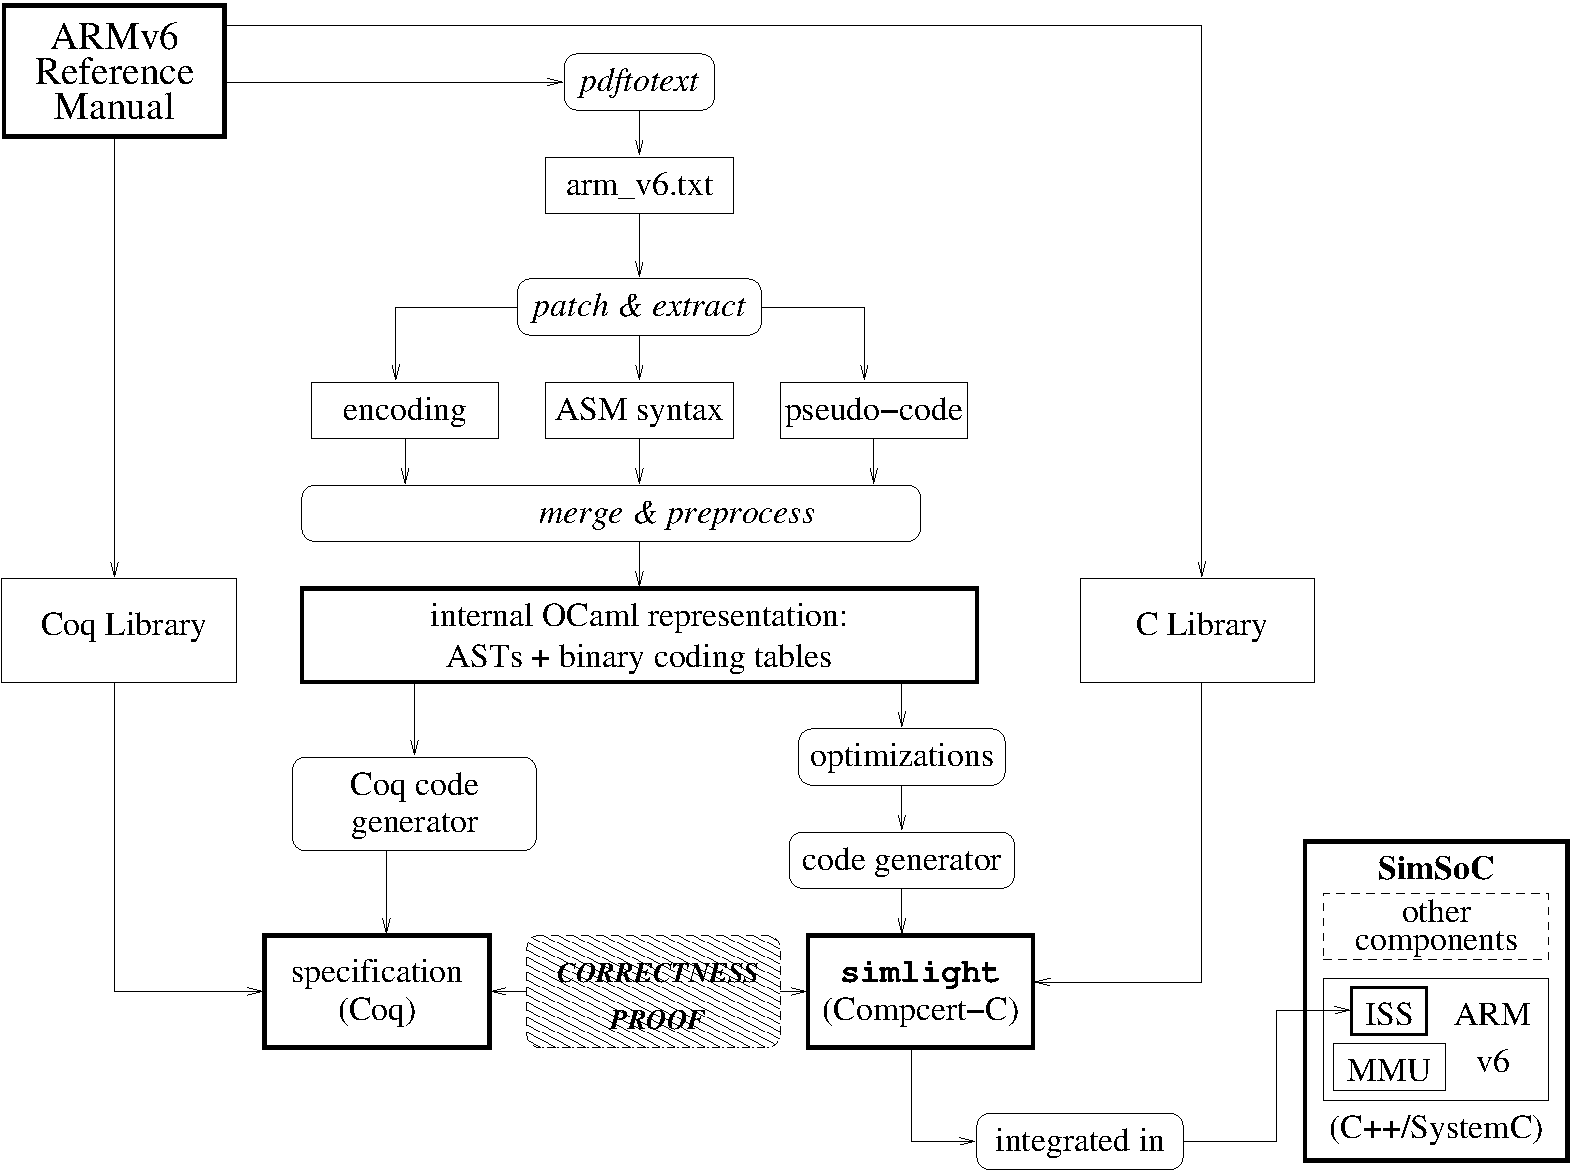
\includegraphics[width=.8\linewidth]{fullarchi.pdf}
\end{frame}

%%%%%%%%%%%%%%%%%%%%%%%%%%%%%%%%%%%%%%%%%%%%%%%%%%%

%\begin{frame}
%\frametitle{Correctness proof}
%\hfil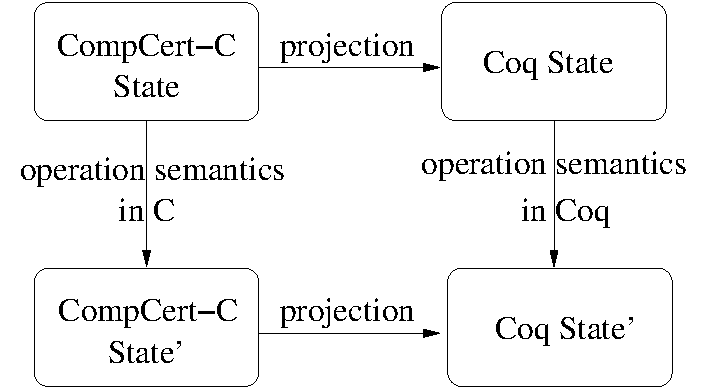
\includegraphics[width=.8\linewidth]{theorem.pdf}
%\end{frame}

%%%%%%%%%%%%%%%%%%%%%%%%%%%%%%%%%%%%%%%%%%%%%%%%%%%
%%%%%%%%%%%%%%%%%%%%%%%%%%%%%%%%%%%%%%%%%%%%%%%%%%%
\section{ARM model}

%%%%%%%%%%%%%%%%%%%%%%%%%%%%%%%%%%%%%%%%%%%%%%%%%%%
\subsection*{...}
\begin{frame}[fragile]
\frametitle{ARMv6 ref manual: instruction ADC in pseudo-code}
%code of ADC
\begin{alltt}
A4.1.2 ADC
  \bleu{if} ConditionPassed(cond) \bleu{then}
    \textbf{Rd = Rn + shifter_operand + C Flag;}
    \bleu{if} S == 1 and d == 15 \bleu{then}
      \bleu{if} CurrentModeHasSPSR() \bleu{then}
          CPSR = SPSR;
      \bleu{else} UNPREDICTABLE
    \bleu{else} \bleu{if} S == 1 \bleu{then}
      N Flag = Rd[31];
      Z Flag = \bleu{if} Rd == 0 \bleu{then} 1 \bleu{else} 0;
      C Flag = CarryFrom(Rn + shifter_operand
                            + C Flag);
      V Flag = OverflowFrom(Rn + shifter_operand
                               + C Flag);

\end{alltt}
\end{frame}

%%%%%%%%%%%%%%%%%%%%%%%%%%%%%%%%%%%%%%%%%%%%%%%%%%%
\subsection{ARM instruction in Coq Specification}
\begin{frame}[fragile]
\frametitle{Coq specification of ADC}
%code of ADC
\small
\begin{alltt}
(* A4.1.2 ADC *)
Definition ADC_step
    (S : bool) (cond : opcode) (d : regnum) (n : regnum)
    (shifter_operand : word) : semfun _ := 
  \brique{<s0>} \bleu{if}_\bleu{then} (ConditionPassed s0 cond)
    ([ \brique{<st>} set_reg d (add (add (reg_content s0 n)
                                shifter_operand)
                                ((cpsr st)[Cbit]))
    ; \bleu{If} (andb (zeq S 1) (zeq d 15))
       \bleu{then}
           (\brique{<st>} if_CurrentModeHasSPSR (fun em =>
              (\brique{<st>} set_cpsr (spsr st em))))
\tiny
            \bleu{else}         (\bleu{if_then} (zeq S 1)
                ([ \brique{<st>} set_cpsr_bit Nbit ((reg_content st d)[n31])
                ; \brique{<st>} set_cpsr_bit Zbit (\bleu{if} zeq (reg_content st d) 0 \bleu{then} repr 1 
                                          \bleu{else} repr 0)
                ; \brique{<st>} set_cpsr_bit Cbit
                          (CarryFrom_add3 (reg_content s0 n) shifter_operand
                                          ((cpsr st)[Cbit]))
                ; \brique{<st>} set_cpsr_bit Vbit (OverflowFrom_add3 (reg_content s0 n)
                                     shifter_operand ((cpsr st)[Cbit])) ])) ]).
\end{alltt}
\end{frame}



%%%%%%%%%%%%%%%%%%%%%%%%%%%%%%%%%%%%%%%%%%%%%%%%%%%

\begin{frame}
\frametitle{Compcert-C}
\begin{block}{Compcert}
Coq-certified C compiler (developed at INRIA)
\end{block}

\bigskip

\begin{block}{Used in SimSoC-Cert}
\begin{itemize}
\item Front-end: operational semantics of a large subset of C
\item Libraries on word arithmetical and logical operations
\end{itemize}
\end{block}

\end{frame}

%%%%%%%%%%%%%%%%%%%%%%%%%%%%%%%%%%%%%%%%%%%%%%%%%%%

\subsection{ARM instruction in Simlight (CompcertC)}
\begin{frame}[fragile]
\frametitle{ADC implementation in Simlight (CompcertC)}
%code of ADC

\small
\begin{alltt}
\bleu{void} ADC(struct SLv6\_Processor *proc,
    \bleu{const} bool S,  \bleu{const} SLv6\_Condition cond,
    \bleu{const} uint8\_t d,  \bleu{const} uint8\_t n,
    \bleu{const} uint32\_t sh\bleu{if}ter\_operand)
\{
\bleu{const} uint32\_t old\_Rn = reg(proc,n);
\bleu{if} (ConditionPassed(&proc->cpsr, cond)) \{
 set\_reg\_or\_pc(proc,d,
   ((old\_Rn + shifter\_operand) + proc->cpsr.C\_flag));
 \bleu{if} (((S == 1) && (d == 15))) \{
  \bleu{if} (CurrentModeHasSPSR(proc))
   copy\_StatusRegister(&proc->cpsr, spsr(proc));
  {}\bleu{else} unpredictable();
\tiny
  \} \bleu{else} \{
   \bleu{if} ((S == 1)) \{
    proc->cpsr.N\_flag = get\_bit(reg(proc,d),31);
    proc->cpsr.Z\_flag = ((reg(proc,d) == 0)? 1: 0);
    proc->cpsr.C\_flag = 
     CarryFrom\_add3(old\_Rn, shifter\_operand, proc->cpsr.C\_flag);
    proc->cpsr.V\_flag = 
     OverflowFrom\_add3(old\_Rn, shifter\_operand, proc->cpsr.C\_flag);
\} \} \} \}
\end{alltt}

\end{frame}

\begin{frame}[fragile]
\frametitle{Coq representation of CompcertC AST}
\newcommand{\mycirc}{\begin{math}\circ\end{math}}
\newcommand{\tbs}{\textbackslash}
\newcommand{\mabullet}{\begin{math}\bullet\end{math}}
\small
\begin{alltt}
Definition ADC\_Coq\_simlight := (ADC, Internal 
    \{| fn_return := void; fn_params := \tiny
         [proc -: `*` typ_SLv6_Processor; 
          S -: uint8; cond -: int32; d -: uint8; n -: uint8; 
          shifter_operand -: uint32];
         fn_vars := [ old_Rn -: uint32];\small
      fn_body :=
($ old_Rn`:\mycirc) `= (call (\tbs{}reg`:\mycirc) E[\tbs{}proc`:\mycirc; \tbs{}n`:\mycirc] \mycirc)`:\mycirc;;
\bleu{`if}\,(\mabullet\,(\tbs{}ConditionPassed`:\mycirc)\,E[&((`*(\tbs{}proc`:\mycirc)`:\mycirc)|cpsr`:\mycirc)`:\mycirc;\,\tbs{}cond`:\mycirc] \mycirc)
 \bleu{then} (\mabullet\,(\tbs{}set_reg_or_pc`:\mycirc) E[\tbs{}proc`:\mycirc; \tbs{}d`:\mycirc; ((\tbs{}old_Rn`:\mycirc)+\mabullet)+\mabullet:\mycirc]\,\mycirc);;
 \bleu{`if} ((($ S`:\mycirc)==(#1`:\mycirc)`:\mycirc)&(($ d`:\mycirc)==(#15`:\mycirc)`:\mycirc)`:\mycirc)\tiny
     \bleu{then} \bleu{`if} (call (\tbs{}CurrentModeHasSPSR`:\mycirc) E[\tbs{}proc`:\mycirc] \mycirc)
      \bleu{then} (call (\tbs{}copy_StatusRegister`:\mycirc) E[&(\mabullet|cpsr`:\mycirc)`:\mycirc; \mabullet] \mycirc)
      \bleu{else} (call ($ unpredictable`:\mycirc) E[] \mycirc)
     \bleu{else} \bleu{`if} (($ S`:\mycirc)==(#1`:\mycirc)`:\mycirc)
      \bleu{then} ((($ proc`:\mycirc)|cpsr`:\mycirc)|N_flag`:\mycirc) `= 
       (\mabullet\,(\tbs{}get_bit`:\mycirc) E[(\mabullet\,(\tbs{}reg`:\mycirc) E[\tbs{}proc`:\mycirc; \tbs{}d`:\mycirc] \mycirc); #31`:\mycirc] \mycirc)`:\mycirc;;
           ((($ proc`:\mycirc)|cpsr`:\mycirc)|Z_flag`:\mycirc) `= 
       (((\mabullet (\tbs{}reg`:\mycirc) \mabullet \mycirc)==(#0`:\mycirc)`:\mycirc)?(#1`:\mycirc)`:(#0`:\mycirc)`:\mycirc)`:\mycirc;;
           ((($ proc`:\mycirc)|cpsr`:\mycirc)|C_flag`:\mycirc) `= 
       (\mabullet (\tbs{}CarryFrom_add3`:\mycirc) E[\mabullet; \mabullet; (\mabullet (\mabullet|C_flag`:\mycirc) \mycirc)] \mycirc)`:\mycirc;;
           ((($ proc`:\mycirc)|cpsr`:\mycirc)|V_flag`:\mycirc) `= 
       (\mabullet (\tbs{}OverflowFrom_add3`:\mycirc) E[(\mabullet (\tbs{}old_Rn`:\mycirc) \mycirc); \mabullet; \mabullet] \mycirc)`:\mycirc
   \bleu{else} skip
 \bleu{else} skip |\}).
\end{alltt}
\end{frame}
%$

%%%%%%%%%%%%%%%%%%%%%%%%%%%%%%%%%%%%%%%%%%%%%%%%%%%

\subsection{Difference}
\begin{frame}
\frametitle{Differences between the two representations}
\begin{block}{Different data types}
More complex types in Simlight, for example:\\
In Coq model, CPSR is a 32 bits word;
in Simlight, CPSR is a data structure, 1 byte-field for every significant bit
\end{block}
\begin{block}{Different semantics}
In Coq specification, semantics is a function\\
In Compcert-C, semantics is a relation.
\end{block}
\begin{block}{Semantics operates on different memory models}
In Coq model, semantics operates directly on processor state\\
In Compcert-C, semantics is related to C memory state where processor state is stored
\end{block}
\end{frame}

%%%%%%%%%%%%%%%%%%%%%%%%%%%%%%%%%%%%%%%%%%%%%%%%%%%
%%%%%%%%%%%%%%%%%%%%%%%%%%%%%%%%%%%%%%%%%%%%%%%%%%%
\section{Correctness proofs}

%%%%%%%%%%%%%%%%%%%%%%%%%%%%%%%%%%%%%%%%%%%%%%%%%%%
\begin{frame}
\frametitle{Correctness of an operation}
\hfil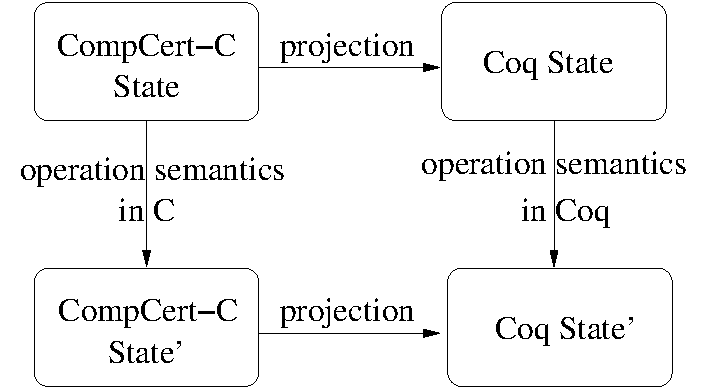
\includegraphics[width=.8\linewidth]{theorem.pdf}
%recall the theorem diagram
\end{frame}

\subsection{Projection of ARMv6 processor state}
\begin{frame}
\frametitle{Projection of ARMv6 processor state ~~(excerpt)}
\hfil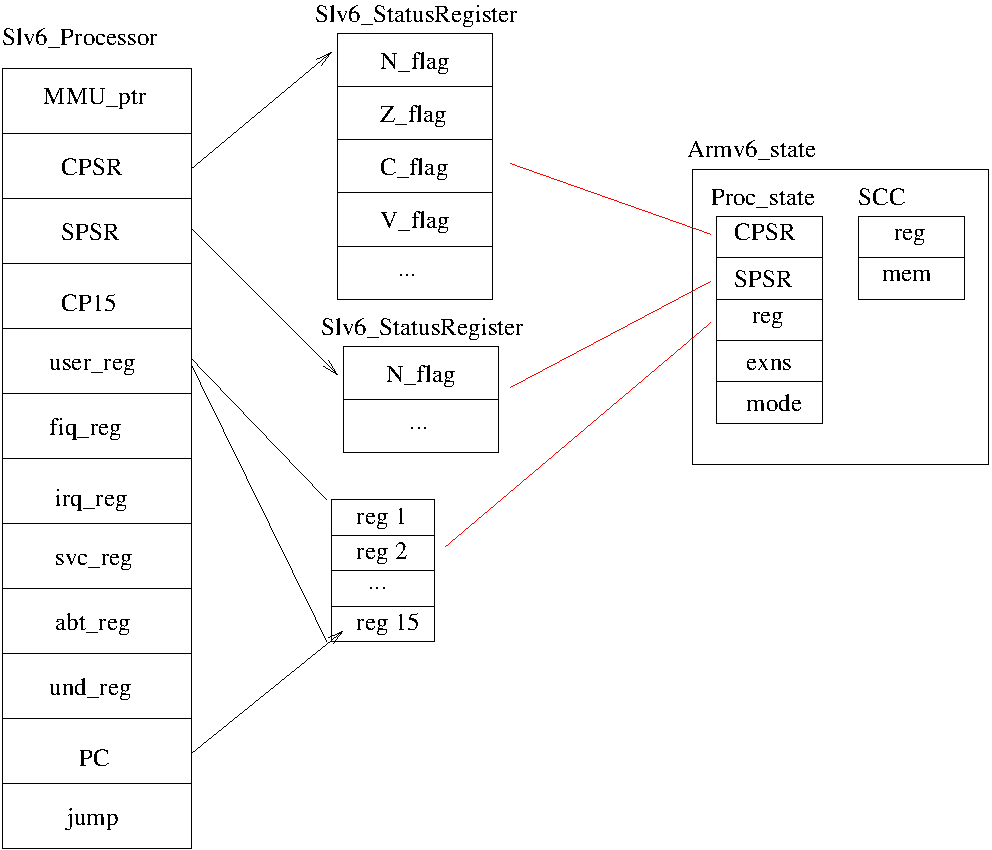
\includegraphics[width=.8\linewidth]{projection.pdf}
\end{frame}

\subsection{Main theorem on ADC}
\begin{frame}
\frametitle{Main theorem on ADC}

\hfil\brique{\emph{\large Pitfall!}}
\bigskip
\begin{theorem}
\begin{itemize}
\item $G,empty\_env\vdash \texttt{alloc\_variables},\brique{M0}\overset{vars}{\Rightarrow}\brique{M1},E$
\item $G,E \vdash \texttt{bind\_parameters},\brique{M1} \overset{vargs}{\Rightarrow}\cvert{M}$
\item $\mathit{proc\_state\_related} \: \cvert{M} \: (\texttt{Ok}\: st)$
\item similarly for the arguments of \texttt{ADC}
\item 
  $G,E\vdash \texttt{ADC\_Coq\_simlight},\cvert{M}\overset{t}{\Rightarrow}out,\cvert{M'}$
\end{itemize}
then $\mathit{proc\_state\_related}\: \cvert{M'} \:(\texttt{ADC\_Coq}\: (\mathit{arguments},\:st))$.
\end{theorem}
\end{frame}

\begin{frame}[fragile]
\frametitle{General proof steps}
\small
\begin{alltt}
e : env; m0 m1 m2 m3 mfin : Memory.mem; s : Arm.state
...
al : alloc_variables empty_env m0 ... m1
bi : bind_parameters e m1 ... vargs m2
psrel : proc_state_related (of_mem proc \cvert{m2}) e
          (Ok tt \{\!| loc := nil; bo := true; st := s |\!\})
...
rn_assgnt : exec_stmt (Genv.globalenv prog_adc) e \cvert{m2}
              (Sdo (Eassign (Evar old_Rn T1)
                      (Ecall (Evalof (Evar reg T2) T2)
                         ...
                         T1) T1)) Events.E0 \cvert{m3} Out_normal
main_p : exec_stmt ... Events.E0 \cvert{mfin} out 
=========================================================
proc_state_related (of_mem proc \cvert{mfin}) e
 (S.ADC_step\;sbit\;cond\;d\;n\;so\;\{\!|\:loc\;:=\;nil;\;bo\;:=\;true;\;st\;:=\;s\:|\!\})

\textbf{thm_ADC <} \brique{my\_inversion} rn_assgnt.

\end{alltt}
\end{frame}

\begin{frame}[fragile]
\frametitle{Conditional expressions in pseudo-code}
%code of ADC
\begin{alltt}
A4.1.2 ADC
  if \brique{ConditionPassed(cond)} then
    Rd = Rn + shifter_operand + C Flag;
    if \brique{S == 1 and d == 15} then
      if CurrentModeHasSPSR() then
          CPSR = SPSR;
      else UNPREDICTABLE
    else if \brique{S == 1} then
      N Flag = Rd[31];
      Z Flag = if Rd == 0 then 1 else 0;
      C Flag = CarryFrom(Rn + shifter_operand
                            + C Flag);
      V Flag = OverflowFrom(Rn + shifter_operand
                               + C Flag);

\end{alltt}
\end{frame}

\subsection{Lemmas}
\begin{frame}
\frametitle{5 groups of lemmas (I)}
%4 groups of lemmasFor internal functions,
\begin{lem}
if $G,E\vdash \texttt{condition}_C ? a1 : a2, M\overset{E0}{\Rightarrow}vres,M'$,\\
then M=M'.
\end{lem}
\begin{lem}
if $G,E\vdash \texttt{condition}_C ? a1 : a2, M\overset{E0}{\Rightarrow}vres,M'$:\\
- and $bool\_val~vres$ = $condition_{Coq}$.
\end{lem}
\end{frame}


\begin{frame}[fragile]
\frametitle{Internal functions in pseudo-code}
%code of ADC
\begin{alltt}
A4.1.2 ADC
  if ConditionPassed(cond) then
    Rd = Rn + shifter_operand + C Flag;
    if S == 1 and d == 15 then
      if CurrentModeHasSPSR() then
          CPSR = SPSR;
      else UNPREDICTABLE
    else if S == 1 then
      N Flag = Rd[31];
      Z Flag = if Rd == 0 then 1 else 0;
      C Flag = \brique{CarryFrom}(Rn + shifter_operand
                            + C Flag);
      V Flag = \brique{OverflowFrom}(Rn + shifter_operand
                               + C Flag);

\end{alltt}
\end{frame}

\begin{frame}
\frametitle{5 groups of lemmas (II)}
\begin{lem}
If $\mathit{proc\_state\_related} \:M~(\texttt{Ok}~st)$,\\ 
and if
$G,E\vdash \texttt{set\_reg}_c(proc,reg\_id,data), M\overset{E0}{\Rightarrow}vres,M'$,\\
then $\mathit{proc\_state\_related}~ M'~ (\texttt{set\_reg}_{Coq}~st)$.
\end{lem}
\begin{lem}
if 
$G,E\vdash \texttt{set\_reg}_c(proc,reg\_id,data), M\overset{E0}{\Rightarrow}vres,M'$,\\
then $P(M)=P(M')$.
\end{lem}
\begin{lem}
if 
$G,E\vdash \texttt{CarryFrom}_c(x,n), M\overset{E0}{\Rightarrow}vres,M'$,\\
then $vres = \texttt{CarryFrom}_{Coq}~x~n$.
\end{lem}
\end{frame}

\subsection{Using Ltac to automate proof steps}
\begin{frame}
\frametitle{Using Ltac to automate proof steps}
%inversion?
We use the big-step semantics defined in CompCert-C, 
a big inductive type with 16 constructors.
\begin{block}
{repetitive proof steps}
If we have

\medskip
Hypothesis\texttt{ ev:eval\_expr e m expression t m'}

\medskip
To get the evolution between m and m', we have to do

\medskip
\texttt{\brique{inversion} ev as [ev' ...].\\\brique{inversion} ev' as [ev'' ...]}\\
...
\end{block}
Solved in one step by \texttt{\cvert{inv\_eval\_expr\_between m m'}}
\end{frame}

%%%%%%%%%%%%%%%%%%%%%%%%%%%%%%%%%%%%%%%%%%
\section{Conclusion}

%%%%%%%%%%%%%%%%%%%%%%%%%%%%%%%%%%%%%%%%%%%%%

\subsection{Size of development}
\begin{frame}
\frametitle{Size of development}
%diagram in paper, add loc of projection

\begin{table}[t]
  \centering
  \begin{tabular}{|l|r@{}l@{~}|}
    \hline 
  % "wc -l" tested with svn revision : 1602
    Original ARM ref man (txt)                        & 50& \\ % wc -l arm6/arm6.txt
    ARM Parsing to an OCaml AST                       & \bleu{1}& \\ % wc -l arm6/parsing/*{ml,sh}
    Generator (Simgen) for ARM and SH4 model          & \bleu{10}& \\ % wc -l simgen/*{ml,v,mly,mll}
    General Coq libraries on ARM                      & 1&.5 \\ % wc -l arm6/coq/*v
    Generated C code for Simlight ARM operations      & \cvert{7}& \\ % wc -l arm6/simlight/slv6_iss.c
    Generated Coq code for ARM operations             & \cvert{2}& \\
    Generated Coq code for ARM decoding               & \cvert{0}&\cvert{.6} \\
    Projection definitions                            & 0&.4\\
    Proof script on \texttt{ADC}                      & \brique{1}& \\ 
    Proof script on library functions                 & \brique{1}&\\
    Ltac definitions                                  & \brique{0}&\brique{.4}\\
    \hline 
  \end{tabular}
  \smallskip
  \caption{Sizes (in Kloc)}
  \label{tab:sizes}
\end{table}
\end{frame}

\subsection{Future work}
\begin{frame}
\frametitle{Future work}
\begin{itemize}
\item Finish the proof for all library functions
\item Extend the work for ADC to other instructions
\item Proofs for decoder
\item Proofs for simulation loop
\end{itemize}
\end{frame}

\subsection{Related work}
\begin{frame}
\frametitle{Related work}
\begin{block}
{Fully manual formalized ARMv7 architecture in HOL4}
To prove hardware or microcode implementation of ARM operations are correct
\end{block}
\bigskip
\begin{block}
{Formalized 2 commercial microprocessors in ACL2}
\begin{itemize}
\item
To prove the correctness of CAP microcode programs
\item
To prove the correctness of the kernel of the floating-point division operation
on AMD5k86
\end{itemize}
\end{block}
%HOL4 formalized ARMv7
%ACL2
\end{frame}


\begin{frame}

\begin{center}

{\huge THANKS}
\end{center}

\end{frame}


\end{document}

